\newcommand{\meshFigIntr}[1]{\includegraphics[width=.100\linewidth,trim=140 10 120 0,clip]{mesh-intro/interpol-#1}}
\newcommand{\imgFigIntr}[1]{\includegraphics[width=.105\linewidth,trim=80 20 80 20,clip]{2d-intro/interpol-ellipses-#1}}

%%% FIG %%%
\begin{figure}\centering
\centering
\HighResFig{
\begin{tabular}{@{\hspace{1mm}}c@{\hspace{1mm}}c@{\hspace{1mm}}c@{\hspace{1mm}}c@{\hspace{1mm}}c@{\hspace{1mm}}c@{\hspace{1mm}}c@{\hspace{1mm}}c@{\hspace{1mm}}c@{}}
\imgFigIntr{1}&
\imgFigIntr{2}&
\imgFigIntr{3}&
\imgFigIntr{4}&
\imgFigIntr{5}&
\imgFigIntr{6}&
\imgFigIntr{7}&
\imgFigIntr{8}&
\imgFigIntr{9}\\
\meshFigIntr{1}&
\meshFigIntr{2}&
\meshFigIntr{3}&
\meshFigIntr{4}&
\meshFigIntr{5}&
\meshFigIntr{6}&
\meshFigIntr{7}&
\meshFigIntr{8}&
\meshFigIntr{9}\\
$t=0$ & $t=1/8$ & $t=1/4$ & $t=3/8$ & $t=1/2$ & $t=5/8$ & $t=3/4$ & $t=7/8$ & $t=1$ 
\end{tabular}
}{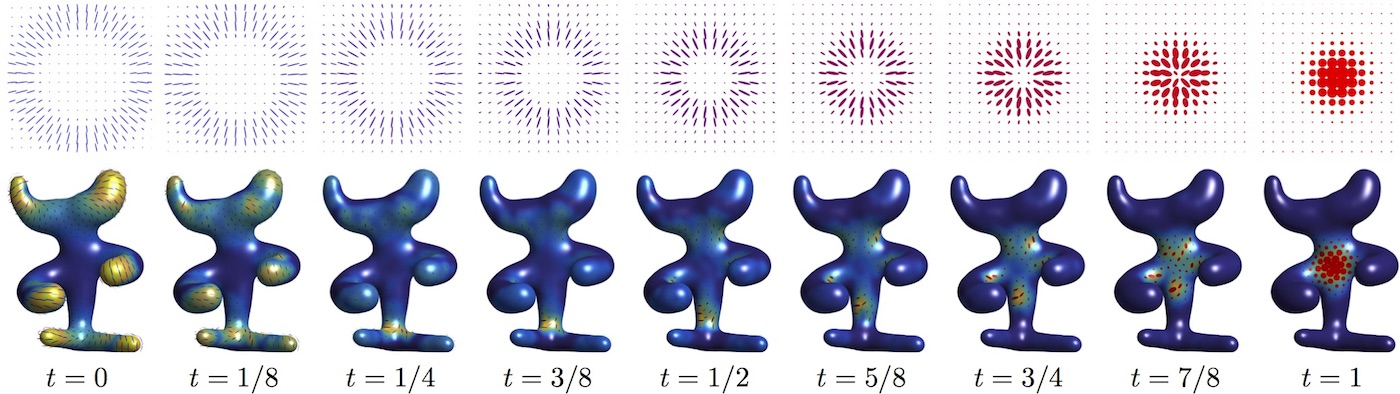
\includegraphics[width=\linewidth]{fig-intro-all.jpg}}
%%%
\caption{%%%
Given two input fields of positive semidefinite matrices (displayed at times $t \in \{0,1\}$ using ellipses) on some domain (here, a 2-D planar square and a surface mesh), our Quantum Optimal Transport (Q-OT) method defines a continuous interpolating path for $t \in [0,1]$. Unlike linear interpolation schemes, Q-OT transports the ``mass'' of the tensors (size of the ellipses) as well as their anisotropy and orientation. This interpolation, and its extension to finding the barycenter of several input fields, is computed using a fast extension of the well-known Sinkhorn algorithm.
} \label{fig:intro}
\end{figure}
%%% FIG %%%

